\documentclass[tikz,border=4pt]{standalone}
\usepackage{tikz}
\usetikzlibrary{arrows.meta}
\definecolor{nebula}{HTML}{6366F1}
\definecolor{spark}{HTML}{14B8A6}
\begin{document}
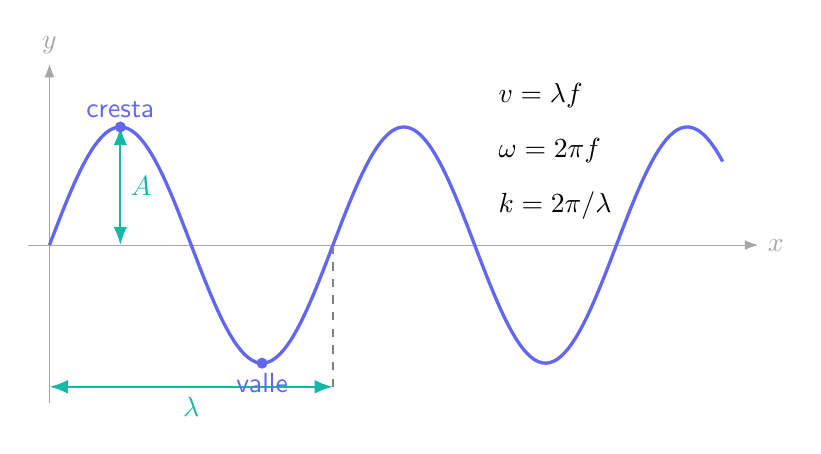
\begin{tikzpicture}[x=.9cm,y=1cm,font=\sffamily,>=Latex]
  \draw[->,gray!70] (-.3,0)--(10,0) node[right] {$x$};
  \draw[->,gray!70] (0,-2)--(0,2.3) node[above] {$y$};
  \draw[domain=0:9.5,samples=180,very thick,nebula] plot (\x,{1.5*sin(90*\x)});
  \draw[<->,spark,thick] (0,-1.8)--(4,-1.8) node[midway,below] {$\lambda$};
  \draw[<->,spark,thick] (1,0)--(1,1.5) node[midway,right] {$A$};
  \draw[dashed,gray] (4,-1.8)--(4,0);
  \fill[nebula] (1,1.5) circle (2pt) node[above] {cresta};
  \fill[nebula] (3,-1.5) circle (2pt) node[below] {valle};
  \node[anchor=west] at (6.2,1.9) {$v=\lambda f$};
  \node[anchor=west] at (6.2,1.2) {$\omega=2\pi f$};
  \node[anchor=west] at (6.2,.5) {$k=2\pi/\lambda$};
\end{tikzpicture}
\end{document}
